Per ogni problema è stata analizzata la distribuzione rispetto al numero di valutatori che lo hanno individuato. Le tabelle seguenti mostrano, per ciascun valutatore, se il problema è stato rilevato o meno.
\vspace{0.3cm}

% Tabella 1: Problemi 1-15
\begin{figure}[H]
\centering
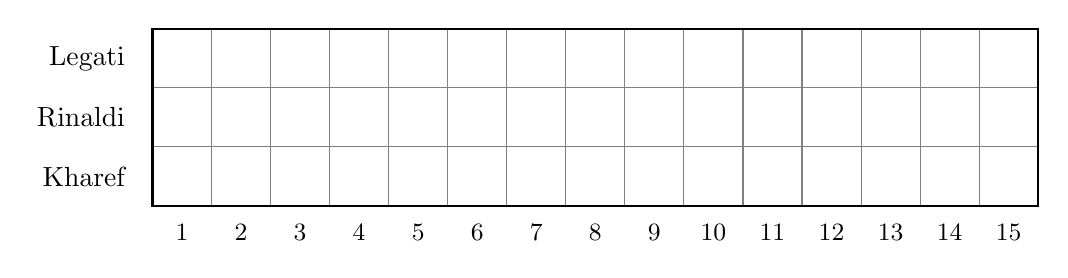
\begin{tikzpicture}[scale=0.75]
    \definecolor{checkcolor}{RGB}{0,0,0}
    
    %\node[anchor=south, font=\large] at (8.5, 4.2) {Problemi 1-15};
    
    % Etichette asse Y
    \node[anchor=east, font=\normalsize] at (0.7, 3.5) {Legati};
    \node[anchor=east, font=\normalsize] at (0.7, 2.5) {Rinaldi};
    \node[anchor=east, font=\normalsize] at (0.7, 1.5) {Kharef};
    
    % Etichette asse X
    \foreach \x in {1,...,15} {
        \node[font=\small] at (\x+0.5, 0.55) {\x};
    }
    
    % Griglia
    \draw[gray!100] (1, 1) grid[step=1] (16, 4);
    \draw[black, thick] (1, 1) rectangle (16, 4);
    
    % Riempimento di default: metto la X rossa ovunque
    \foreach \x in {1,...,15} {
        \node at (\x+0.5, 3.5) {\notfound}; % Riga Legati
        \node at (\x+0.5, 2.5) {\notfound}; % Riga Rinaldi
        \node at (\x+0.5, 1.5) {\notfound}; % Riga Kharef
    }
    
    % Sovrascrivo con la spunta verde DOVE HANNO TROVATO il problema
    
    % Dati - Legati (Trovati)
    \foreach \x in {1,2,3,4,5,6,7,8,9,10,11,12,13,14,15} {
        \node[fill=white, inner sep=1pt] at (\x+0.5, 3.5) {\found};
    }
    
    % Dati - Rinaldi (Trovati)
    \foreach \x in {2,3,5,6,8,9,11,12,13,14} {
        \node[fill=white, inner sep=1pt] at (\x+0.5, 2.5) {\found};
    }
    
    % Dati - Kharef (Trovati)
    \foreach \x in {2,3,5,6,9,11,12,15} {
        \node[fill=white, inner sep=1pt] at (\x+0.5, 1.5) {\found};
    }
\end{tikzpicture}
\end{figure}

% Tabella 2: Problemi 16-30
\begin{figure}[H]
\centering
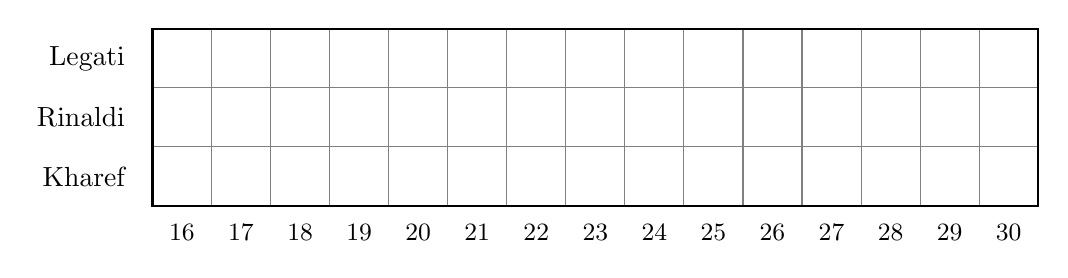
\begin{tikzpicture}[scale=0.75]
    \definecolor{checkcolor}{RGB}{0,0,0}
    
    % Etichette asse Y
    \node[anchor=east, font=\normalsize] at (0.7, 3.5) {Legati};
    \node[anchor=east, font=\normalsize] at (0.7, 2.5) {Rinaldi};
    \node[anchor=east, font=\normalsize] at (0.7, 1.5) {Kharef};
    
    % Etichette asse X
    \foreach \x/\label in {1/16,2/17,3/18,4/19,5/20,6/21,7/22,8/23,9/24,10/25,11/26,12/27,13/28,14/29,15/30} {
        \node[font=\small] at (\x+0.5, 0.55) {\label};
    }
    
    % Griglia
    \draw[gray!100] (1, 1) grid[step=1] (16, 4);
    \draw[black, thick] (1, 1) rectangle (16, 4);
    
    % Default: X rossa
    \foreach \x in {1,...,15} {
        \node at (\x+0.5, 3.5) {\notfound};
        \node at (\x+0.5, 2.5) {\notfound};
        \node at (\x+0.5, 1.5) {\notfound};
    }
    
    % Dati - Legati (Trovati)
    \foreach \x in {2,6,7,8,9,10,11,12,13,14,15} {
        \node[fill=white, inner sep=1pt] at (\x+0.5, 3.5) {\found};
    }
    
    % Dati - Rinaldi (Trovati)
    \foreach \x in {1,2,3,4,6,11,13} {
        \node[fill=white, inner sep=1pt] at (\x+0.5, 2.5) {\found};
    }
    
    % Dati - Kharef (Trovati)
    \foreach \x in {2,6,13} {
        \node[fill=white, inner sep=1pt] at (\x+0.5, 1.5) {\found};
    }
\end{tikzpicture}
\end{figure}

% Tabella 3: Problemi 31-45
\begin{figure}[H]
\centering
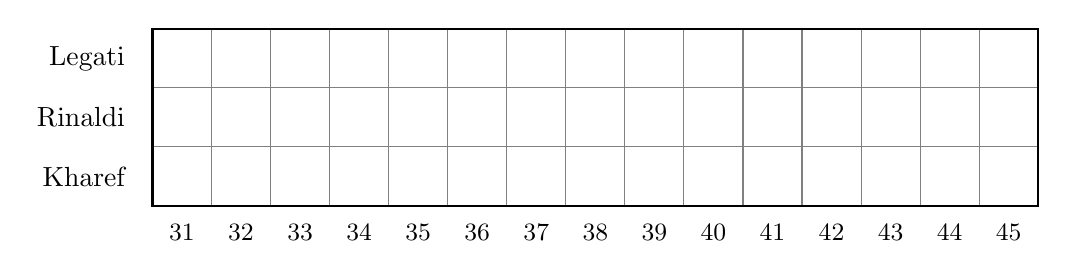
\begin{tikzpicture}[scale=0.75]
    \definecolor{checkcolor}{RGB}{0,0,0}
    
    % Etichette asse Y
    \node[anchor=east, font=\normalsize] at (0.7, 3.5) {Legati};
    \node[anchor=east, font=\normalsize] at (0.7, 2.5) {Rinaldi};
    \node[anchor=east, font=\normalsize] at (0.7, 1.5) {Kharef};
    
    % Etichette asse X
    \foreach \x/\label in {1/31,2/32,3/33,4/34,5/35,6/36,7/37,8/38,9/39,10/40,11/41,12/42,13/43,14/44,15/45} {
        \node[font=\small] at (\x+0.5, 0.55) {\label};
    }
    
    % Griglia
    \draw[gray!100] (1, 1) grid[step=1] (16, 4);
    \draw[black, thick] (1, 1) rectangle (16, 4);
    
    % Default: X rossa
    \foreach \x in {1,...,15} {
        \node at (\x+0.5, 3.5) {\notfound};
        \node at (\x+0.5, 2.5) {\notfound};
        \node at (\x+0.5, 1.5) {\notfound};
    }
    
    % Dati - Legati (Trovati)
    \foreach \x in {1,2,3,4,5,6,7,8,9,10,11,12,13,14,15} {
        \node[fill=white, inner sep=1pt] at (\x+0.5, 3.5) {\found};
    }
    
    % Dati - Rinaldi (Trovati)
    \foreach \x in {3,5,8,10} {
        \node[fill=white, inner sep=1pt] at (\x+0.5, 2.5) {\found};
    }
    
    % Dati - Kharef (Trovati)
    \foreach \x in {5,7,11,13,15} {
        \node[fill=white, inner sep=1pt] at (\x+0.5, 1.5) {\found};
    }
\end{tikzpicture}
\end{figure}

% Tabella 4: Problemi 46-60
\begin{figure}[H]
\centering
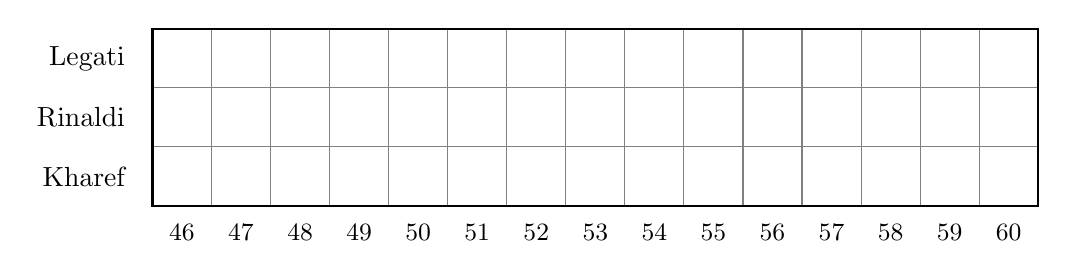
\begin{tikzpicture}[scale=0.75]
    \definecolor{checkcolor}{RGB}{0,0,0}
    
    % Etichette asse Y
    \node[anchor=east, font=\normalsize] at (0.7, 3.5) {Legati};
    \node[anchor=east, font=\normalsize] at (0.7, 2.5) {Rinaldi};
    \node[anchor=east, font=\normalsize] at (0.7, 1.5) {Kharef};
    
    % Etichette asse X
    \foreach \x/\label in {1/46,2/47,3/48,4/49,5/50,6/51,7/52,8/53,9/54,10/55,11/56,12/57,13/58,14/59,15/60} {
        \node[font=\small] at (\x+0.5, 0.55) {\label};
    }
    
    % Griglia
    \draw[gray!100] (1, 1) grid[step=1] (16, 4);
    \draw[black, thick] (1, 1) rectangle (16, 4);
    
    % Default: X rossa
    \foreach \x in {1,...,15} {
        \node at (\x+0.5, 3.5) {\notfound};
        \node at (\x+0.5, 2.5) {\notfound};
        \node at (\x+0.5, 1.5) {\notfound};
    }
    
    % Dati - Legati (Trovati)
    \foreach \x in {1,2,3} {
        \node[fill=white, inner sep=1pt] at (\x+0.5, 3.5) {\found};
    }
    
    % Dati - Rinaldi (Trovati)
    \foreach \x in {3} {
        \node[fill=white, inner sep=1pt] at (\x+0.5, 2.5) {\found};
    }
    
    % Dati - Kharef (Trovati)
    \foreach \x in {4,5,6,7,8,9,10,11,12,13,14,15} {
        \node[fill=white, inner sep=1pt] at (\x+0.5, 1.5) {\found};
    }
\end{tikzpicture}
\end{figure}

% Tabella 5: Problemi 61-75
\begin{figure}[H]
\centering
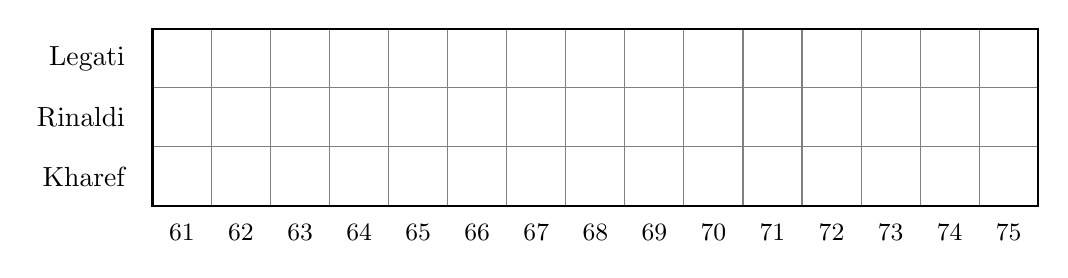
\begin{tikzpicture}[scale=0.75]
    \definecolor{checkcolor}{RGB}{0,0,0}
    
    % Etichette asse Y
    \node[anchor=east, font=\normalsize] at (0.7, 3.5) {Legati};
    \node[anchor=east, font=\normalsize] at (0.7, 2.5) {Rinaldi};
    \node[anchor=east, font=\normalsize] at (0.7, 1.5) {Kharef};
    
    % Etichette asse X
    \foreach \x/\label in {1/61,2/62,3/63,4/64,5/65,6/66,7/67,8/68,9/69,10/70,11/71,12/72,13/73,14/74,15/75} {
        \node[font=\small] at (\x+0.5, 0.55) {\label};
    }
    
    % Griglia
    \draw[gray!100] (1, 1) grid[step=1] (16, 4);
    \draw[black, thick] (1, 1) rectangle (16, 4);
    
    % Default: X rossa
    \foreach \x in {1,...,15} {
        \node at (\x+0.5, 3.5) {\notfound};
        \node at (\x+0.5, 2.5) {\notfound};
        \node at (\x+0.5, 1.5) {\notfound};
    }
    
    % Dati - Kharef (Trovati) - Gli altri due valutatori qui hanno tutte X rosse
    \foreach \x in {1,2,3,4,5,6,7,8,9,10,11,12,13,14,15} {
        \node[fill=white, inner sep=1pt] at (\x+0.5, 1.5) {\found};
    }
\end{tikzpicture}
\end{figure}

% Tabella 6: Problemi 76-93
\begin{figure}[H]
\centering
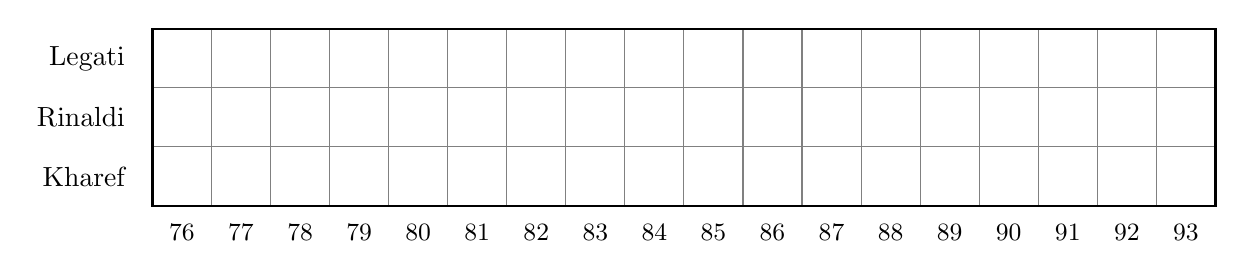
\begin{tikzpicture}[scale=0.75]
    \definecolor{checkcolor}{RGB}{0,0,0}
    
    % Etichette asse Y
    \node[anchor=east, font=\normalsize] at (0.7, 3.5) {Legati};
    \node[anchor=east, font=\normalsize] at (0.7, 2.5) {Rinaldi};
    \node[anchor=east, font=\normalsize] at (0.7, 1.5) {Kharef};
    
    % Etichette asse X
    \foreach \x/\label in {1/76,2/77,3/78,4/79,5/80,6/81,7/82,8/83,9/84,10/85,11/86,12/87,13/88,14/89,15/90,16/91,17/92,18/93} {
        \node[font=\small] at (\x+0.5, 0.55) {\label};
    }
    
    % Griglia
    \draw[gray!100] (1, 1) grid[step=1] (19, 4);
    \draw[black, thick] (1, 1) rectangle (19, 4);
    
    % Default: X rossa
    \foreach \x in {1,...,18} {
        \node at (\x+0.5, 3.5) {\notfound};
        \node at (\x+0.5, 2.5) {\notfound};
        \node at (\x+0.5, 1.5) {\notfound};
    }
    
    % Dati - Rinaldi (Trovati)
    \foreach \x in {5,6,7,8,9,10,11,12,13,14,15,16,17,18} {
        \node[fill=white, inner sep=1pt] at (\x+0.5, 2.5) {\found};
    }
    
    % Dati - Kharef (Trovati)
    \foreach \x in {1,2,3,4,12} {
        \node[fill=white, inner sep=1pt] at (\x+0.5, 1.5) {\found};
    }
\end{tikzpicture}
\end{figure}

\noindent
Sui 93 problemi totali individuati, di cui alcuni sono stati rilevati da più valutatori, la tabella seguente riporta un riepilogo del contributo di ciascun valutatore con le relative percentuali.
% Tabella Riepilogo
\begin{center}
    \renewcommand{\arraystretch}{1.3}
    \begin{tabular}{|l|c|c|}
        \hline
        \textbf{Valutatore} & \textbf{Problemi Identificati} & \textbf{Percentuale} \\
        \hline
        Legati & 44 & $47\%$ \\
        \hline
        Rinaldi & 36 & $38\%$ \\
        \hline
        Kharef & 48 & $52\%$ \\
        \hline
    \end{tabular}
\end{center}

\vspace{0.3cm}

Dall'analisi dei risultati emerge una certa variabilità nel numero di problemi individuati dai diversi valutatori. Si nota in particolare che Kharef ha rilevato più criticità rispetto alla media del gruppo (52\% contro una media del 45\%). 

Questo risultato può essere attribuito al fatto che, avendo sviluppato il sistema, possedeva una conoscenza più approfondita dell'architettura e delle funzionalità di \textit{BrainBox}.

I valutatori hanno identificato in gran parte problemi diversi, con poche sovrapposizioni. 
Questo dimostra l'importanza di utilizzare valutatori con diversi gradi di familiarità 
con il sistema per una valutazione più completa.